% Options for packages loaded elsewhere
% Options for packages loaded elsewhere
\PassOptionsToPackage{unicode}{hyperref}
\PassOptionsToPackage{hyphens}{url}
\PassOptionsToPackage{dvipsnames,svgnames,x11names}{xcolor}
%
\documentclass[
  letterpaper,
  DIV=11,
  numbers=noendperiod]{scrartcl}
\usepackage{xcolor}
\usepackage{amsmath,amssymb}
\setcounter{secnumdepth}{-\maxdimen} % remove section numbering
\usepackage{iftex}
\ifPDFTeX
  \usepackage[T1]{fontenc}
  \usepackage[utf8]{inputenc}
  \usepackage{textcomp} % provide euro and other symbols
\else % if luatex or xetex
  \usepackage{unicode-math} % this also loads fontspec
  \defaultfontfeatures{Scale=MatchLowercase}
  \defaultfontfeatures[\rmfamily]{Ligatures=TeX,Scale=1}
\fi
\usepackage{lmodern}
\ifPDFTeX\else
  % xetex/luatex font selection
\fi
% Use upquote if available, for straight quotes in verbatim environments
\IfFileExists{upquote.sty}{\usepackage{upquote}}{}
\IfFileExists{microtype.sty}{% use microtype if available
  \usepackage[]{microtype}
  \UseMicrotypeSet[protrusion]{basicmath} % disable protrusion for tt fonts
}{}
\makeatletter
\@ifundefined{KOMAClassName}{% if non-KOMA class
  \IfFileExists{parskip.sty}{%
    \usepackage{parskip}
  }{% else
    \setlength{\parindent}{0pt}
    \setlength{\parskip}{6pt plus 2pt minus 1pt}}
}{% if KOMA class
  \KOMAoptions{parskip=half}}
\makeatother
% Make \paragraph and \subparagraph free-standing
\makeatletter
\ifx\paragraph\undefined\else
  \let\oldparagraph\paragraph
  \renewcommand{\paragraph}{
    \@ifstar
      \xxxParagraphStar
      \xxxParagraphNoStar
  }
  \newcommand{\xxxParagraphStar}[1]{\oldparagraph*{#1}\mbox{}}
  \newcommand{\xxxParagraphNoStar}[1]{\oldparagraph{#1}\mbox{}}
\fi
\ifx\subparagraph\undefined\else
  \let\oldsubparagraph\subparagraph
  \renewcommand{\subparagraph}{
    \@ifstar
      \xxxSubParagraphStar
      \xxxSubParagraphNoStar
  }
  \newcommand{\xxxSubParagraphStar}[1]{\oldsubparagraph*{#1}\mbox{}}
  \newcommand{\xxxSubParagraphNoStar}[1]{\oldsubparagraph{#1}\mbox{}}
\fi
\makeatother

\usepackage{color}
\usepackage{fancyvrb}
\newcommand{\VerbBar}{|}
\newcommand{\VERB}{\Verb[commandchars=\\\{\}]}
\DefineVerbatimEnvironment{Highlighting}{Verbatim}{commandchars=\\\{\}}
% Add ',fontsize=\small' for more characters per line
\usepackage{framed}
\definecolor{shadecolor}{RGB}{241,243,245}
\newenvironment{Shaded}{\begin{snugshade}}{\end{snugshade}}
\newcommand{\AlertTok}[1]{\textcolor[rgb]{0.68,0.00,0.00}{#1}}
\newcommand{\AnnotationTok}[1]{\textcolor[rgb]{0.37,0.37,0.37}{#1}}
\newcommand{\AttributeTok}[1]{\textcolor[rgb]{0.40,0.45,0.13}{#1}}
\newcommand{\BaseNTok}[1]{\textcolor[rgb]{0.68,0.00,0.00}{#1}}
\newcommand{\BuiltInTok}[1]{\textcolor[rgb]{0.00,0.23,0.31}{#1}}
\newcommand{\CharTok}[1]{\textcolor[rgb]{0.13,0.47,0.30}{#1}}
\newcommand{\CommentTok}[1]{\textcolor[rgb]{0.37,0.37,0.37}{#1}}
\newcommand{\CommentVarTok}[1]{\textcolor[rgb]{0.37,0.37,0.37}{\textit{#1}}}
\newcommand{\ConstantTok}[1]{\textcolor[rgb]{0.56,0.35,0.01}{#1}}
\newcommand{\ControlFlowTok}[1]{\textcolor[rgb]{0.00,0.23,0.31}{\textbf{#1}}}
\newcommand{\DataTypeTok}[1]{\textcolor[rgb]{0.68,0.00,0.00}{#1}}
\newcommand{\DecValTok}[1]{\textcolor[rgb]{0.68,0.00,0.00}{#1}}
\newcommand{\DocumentationTok}[1]{\textcolor[rgb]{0.37,0.37,0.37}{\textit{#1}}}
\newcommand{\ErrorTok}[1]{\textcolor[rgb]{0.68,0.00,0.00}{#1}}
\newcommand{\ExtensionTok}[1]{\textcolor[rgb]{0.00,0.23,0.31}{#1}}
\newcommand{\FloatTok}[1]{\textcolor[rgb]{0.68,0.00,0.00}{#1}}
\newcommand{\FunctionTok}[1]{\textcolor[rgb]{0.28,0.35,0.67}{#1}}
\newcommand{\ImportTok}[1]{\textcolor[rgb]{0.00,0.46,0.62}{#1}}
\newcommand{\InformationTok}[1]{\textcolor[rgb]{0.37,0.37,0.37}{#1}}
\newcommand{\KeywordTok}[1]{\textcolor[rgb]{0.00,0.23,0.31}{\textbf{#1}}}
\newcommand{\NormalTok}[1]{\textcolor[rgb]{0.00,0.23,0.31}{#1}}
\newcommand{\OperatorTok}[1]{\textcolor[rgb]{0.37,0.37,0.37}{#1}}
\newcommand{\OtherTok}[1]{\textcolor[rgb]{0.00,0.23,0.31}{#1}}
\newcommand{\PreprocessorTok}[1]{\textcolor[rgb]{0.68,0.00,0.00}{#1}}
\newcommand{\RegionMarkerTok}[1]{\textcolor[rgb]{0.00,0.23,0.31}{#1}}
\newcommand{\SpecialCharTok}[1]{\textcolor[rgb]{0.37,0.37,0.37}{#1}}
\newcommand{\SpecialStringTok}[1]{\textcolor[rgb]{0.13,0.47,0.30}{#1}}
\newcommand{\StringTok}[1]{\textcolor[rgb]{0.13,0.47,0.30}{#1}}
\newcommand{\VariableTok}[1]{\textcolor[rgb]{0.07,0.07,0.07}{#1}}
\newcommand{\VerbatimStringTok}[1]{\textcolor[rgb]{0.13,0.47,0.30}{#1}}
\newcommand{\WarningTok}[1]{\textcolor[rgb]{0.37,0.37,0.37}{\textit{#1}}}

\usepackage{longtable,booktabs,array}
\usepackage{calc} % for calculating minipage widths
% Correct order of tables after \paragraph or \subparagraph
\usepackage{etoolbox}
\makeatletter
\patchcmd\longtable{\par}{\if@noskipsec\mbox{}\fi\par}{}{}
\makeatother
% Allow footnotes in longtable head/foot
\IfFileExists{footnotehyper.sty}{\usepackage{footnotehyper}}{\usepackage{footnote}}
\makesavenoteenv{longtable}
\usepackage{graphicx}
\makeatletter
\newsavebox\pandoc@box
\newcommand*\pandocbounded[1]{% scales image to fit in text height/width
  \sbox\pandoc@box{#1}%
  \Gscale@div\@tempa{\textheight}{\dimexpr\ht\pandoc@box+\dp\pandoc@box\relax}%
  \Gscale@div\@tempb{\linewidth}{\wd\pandoc@box}%
  \ifdim\@tempb\p@<\@tempa\p@\let\@tempa\@tempb\fi% select the smaller of both
  \ifdim\@tempa\p@<\p@\scalebox{\@tempa}{\usebox\pandoc@box}%
  \else\usebox{\pandoc@box}%
  \fi%
}
% Set default figure placement to htbp
\def\fps@figure{htbp}
\makeatother





\setlength{\emergencystretch}{3em} % prevent overfull lines

\providecommand{\tightlist}{%
  \setlength{\itemsep}{0pt}\setlength{\parskip}{0pt}}



 


\usepackage{fvextra}
\DefineVerbatimEnvironment{Highlighting}{Verbatim}{breaklines,breakanywhere,commandchars=\\\{\}}
\KOMAoption{captions}{tableheading}
\makeatletter
\@ifpackageloaded{caption}{}{\usepackage{caption}}
\AtBeginDocument{%
\ifdefined\contentsname
  \renewcommand*\contentsname{Table of contents}
\else
  \newcommand\contentsname{Table of contents}
\fi
\ifdefined\listfigurename
  \renewcommand*\listfigurename{List of Figures}
\else
  \newcommand\listfigurename{List of Figures}
\fi
\ifdefined\listtablename
  \renewcommand*\listtablename{List of Tables}
\else
  \newcommand\listtablename{List of Tables}
\fi
\ifdefined\figurename
  \renewcommand*\figurename{Figure}
\else
  \newcommand\figurename{Figure}
\fi
\ifdefined\tablename
  \renewcommand*\tablename{Table}
\else
  \newcommand\tablename{Table}
\fi
}
\@ifpackageloaded{float}{}{\usepackage{float}}
\floatstyle{ruled}
\@ifundefined{c@chapter}{\newfloat{codelisting}{h}{lop}}{\newfloat{codelisting}{h}{lop}[chapter]}
\floatname{codelisting}{Listing}
\newcommand*\listoflistings{\listof{codelisting}{List of Listings}}
\makeatother
\makeatletter
\makeatother
\makeatletter
\@ifpackageloaded{caption}{}{\usepackage{caption}}
\@ifpackageloaded{subcaption}{}{\usepackage{subcaption}}
\makeatother
\usepackage{bookmark}
\IfFileExists{xurl.sty}{\usepackage{xurl}}{} % add URL line breaks if available
\urlstyle{same}
\hypersetup{
  pdftitle={Intermediate Elective 2},
  pdfauthor={Rebecca Martinez},
  colorlinks=true,
  linkcolor={blue},
  filecolor={Maroon},
  citecolor={Blue},
  urlcolor={Blue},
  pdfcreator={LaTeX via pandoc}}


\title{Intermediate Elective 2}
\author{Rebecca Martinez}
\date{2026-05-15}
\begin{document}
\maketitle


\section{1. Inspiration}\label{inspiration}

\subsection{Visualization inspiration}\label{visualization-inspiration}

I chose Steven Ponce's ``Coal falls. Renewables rise.'' as my
inspiration. I liked how the visualization uses two directly labeled
time series lines, a dark background, and contrasting colors to show two
categories changing through time. I also liked that the color contrast
helps separate a less desirable trend from a more desirable one, which
fits my goal of comparing non-native and native vegetation cover in
vernal pools.

\subsection{Why it makes sense for my
dataset}\label{why-it-makes-sense-for-my-dataset}

This inspiration makes sense for my dataset because the vernal pool
vegetation data include percent cover values across multiple years.
Since I am interested in comparing native and non-native vegetation
cover through time, a two-line time series is a good way to show whether
these groups follow similar or contrasting patterns.

\subsection{Variables and visual
mapping}\label{variables-and-visual-mapping}

The x-axis will show year, and the y-axis will show mean percent cover
across vernal pools. The \texttt{cover\_group} variable will be mapped
to color so native and non-native vegetation are shown as separate
lines. Points will show yearly values, lines will show the trend through
time, and direct labels/annotations will help emphasize the contrast
between native and non-native cover.

\section{2. Planned figure}\label{planned-figure}

The sketch below shows the planned layout for my figure. It includes two
time series lines, direct labels for native and non-native cover, and a
dark background inspired by the original visualization.

\begin{figure}[H]

{\centering \pandocbounded{\includegraphics[keepaspectratio]{../images/sketch.jpg}}

}

\caption{planned\_figure}

\end{figure}%

\section{3. Code the figure}\label{code-the-figure}

\subsection{Setup}\label{setup}

\subsubsection{Packages}\label{packages}

\begin{Shaded}
\begin{Highlighting}[]
\CommentTok{\# general use}
\FunctionTok{library}\NormalTok{(tidyverse)}
\FunctionTok{library}\NormalTok{(janitor) }\CommentTok{\# clean column names}

\CommentTok{\# file organization}
\FunctionTok{library}\NormalTok{(here)}

\CommentTok{\# data visualization}
\FunctionTok{library}\NormalTok{(naniar) }\CommentTok{\# visualize missing data}
\FunctionTok{library}\NormalTok{(patchwork) }\CommentTok{\# arrange plots}
\FunctionTok{library}\NormalTok{(viridis) }\CommentTok{\# color palette}
\end{Highlighting}
\end{Shaded}

\subsubsection{Data}\label{data}

\begin{Shaded}
\begin{Highlighting}[]
\CommentTok{\# read in vegetation data}
\NormalTok{veg }\OtherTok{\textless{}{-}} \FunctionTok{read\_csv}\NormalTok{(}\FunctionTok{here}\NormalTok{(}\StringTok{"data"}\NormalTok{, }\StringTok{"veg.csv"}\NormalTok{))}

\CommentTok{\# read in vernal pool vegetation metadata}
\NormalTok{metadata }\OtherTok{\textless{}{-}} \FunctionTok{read\_csv}\NormalTok{(}\FunctionTok{here}\NormalTok{(}\StringTok{"data"}\NormalTok{, }\StringTok{"vp\_veg\_metadata.csv"}\NormalTok{))}
\end{Highlighting}
\end{Shaded}

\subsection{Cleaning}\label{cleaning}

\subsubsection{Create explicit 0s}\label{create-explicit-0s}

\begin{Shaded}
\begin{Highlighting}[]
\CommentTok{\# create explicit{-}zero data frame by species}
\NormalTok{pools\_explicit0 }\OtherTok{\textless{}{-}}\NormalTok{ veg }\SpecialCharTok{|\textgreater{}} 
  
  \CommentTok{\# keep only vernal pool transects at NCOS}
  \FunctionTok{filter}\NormalTok{(}\FunctionTok{str\_detect}\NormalTok{(transect\_name, }\StringTok{"VP"}\NormalTok{) }\SpecialCharTok{\&}
\NormalTok{           site }\SpecialCharTok{==} \StringTok{"ncos"}\NormalTok{) }\SpecialCharTok{|\textgreater{}} 
  
  \CommentTok{\# add missing combinations and fill missing percent cover with 0}
  \FunctionTok{complete}\NormalTok{(year,}
\NormalTok{           transect\_name,}
\NormalTok{           psoc,}
\NormalTok{           transect\_distance,}
           \AttributeTok{fill =} \FunctionTok{list}\NormalTok{(}\AttributeTok{percent\_cover =} \DecValTok{0}\NormalTok{)) }\SpecialCharTok{|\textgreater{}} 
  
  \CommentTok{\# group by year, transect, and species}
  \FunctionTok{group\_by}\NormalTok{(year, transect\_name, psoc) }\SpecialCharTok{|\textgreater{}} 
  
  \CommentTok{\# calculate total percent cover}
  \FunctionTok{summarize}\NormalTok{(}\AttributeTok{sum\_pc =} \FunctionTok{sum}\NormalTok{(percent\_cover, }\AttributeTok{na.rm =} \ConstantTok{TRUE}\NormalTok{),}
            \AttributeTok{.groups =} \StringTok{"drop"}\NormalTok{) }\SpecialCharTok{|\textgreater{}} 
  
  \CommentTok{\# create a shared column for joining with metadata}
  \CommentTok{\# keep year and transect\_name because we need them later}
  \FunctionTok{unite}\NormalTok{(}\StringTok{"year\_pool"}\NormalTok{,}
\NormalTok{        year,}
\NormalTok{        transect\_name,}
        \AttributeTok{remove =} \ConstantTok{FALSE}\NormalTok{) }\SpecialCharTok{|\textgreater{}} 
  
  \CommentTok{\# join metadata to add number of quadrats}
  \FunctionTok{left\_join}\NormalTok{(metadata }\SpecialCharTok{|\textgreater{}}
              \FunctionTok{select}\NormalTok{(year\_pool, num\_quad),}
            \AttributeTok{by =} \StringTok{"year\_pool"}\NormalTok{) }\SpecialCharTok{|\textgreater{}} 
  
  \CommentTok{\# calculate mean percent cover using number of quadrats}
  \FunctionTok{mutate}\NormalTok{(}\AttributeTok{mean\_pc =}\NormalTok{ sum\_pc }\SpecialCharTok{/}\NormalTok{ num\_quad)}

\CommentTok{\# check cleaned data}
\NormalTok{pools\_explicit0 }\SpecialCharTok{|\textgreater{}}
  \FunctionTok{slice\_sample}\NormalTok{(}\AttributeTok{n =} \DecValTok{10}\NormalTok{)}
\end{Highlighting}
\end{Shaded}

\begin{verbatim}
# A tibble: 10 x 7
   year_pool   year transect_name psoc                   sum_pc num_quad mean_pc
   <chr>      <dbl> <chr>         <chr>                   <dbl>    <dbl>   <dbl>
 1 2023_VP-05  2023 VP-05         Medicago_lupulina           2       15   0.133
 2 2025_VP-02  2025 VP-02         Plagiobothrys_undulat~      0       19   0    
 3 2025_VP-01  2025 VP-01         Lactuca_saligna             0       24   0    
 4 2022_VP-07  2022 VP-07         Vicia_sativa                0       19   0    
 5 2022_VP-04  2022 VP-04         Hedypnois_cretica           0       20   0    
 6 2022_VP-02  2022 VP-02         Erigeron_canadensis         0       19   0    
 7 2021_VP-01  2021 VP-01         Sisyrinchium_bellum         0       25   0    
 8 2023_VP-08  2023 VP-08         Distichlis_spicata         16       18   0.889
 9 2021_VP-04  2021 VP-04         Hordeum_brachyantheru~      0       20   0    
10 2023_VP-05  2023 VP-05         Psilocarphus_tennulus       0       15   0    
\end{verbatim}

\begin{Shaded}
\begin{Highlighting}[]
\CommentTok{\# check column names}
\FunctionTok{names}\NormalTok{(pools\_explicit0)}
\end{Highlighting}
\end{Shaded}

\begin{verbatim}
[1] "year_pool"     "year"          "transect_name" "psoc"         
[5] "sum_pc"        "num_quad"      "mean_pc"      
\end{verbatim}

\begin{Shaded}
\begin{Highlighting}[]
\CommentTok{\# check missingness after cleaning}
\FunctionTok{gg\_miss\_var}\NormalTok{(pools\_explicit0)}
\end{Highlighting}
\end{Shaded}

\pandocbounded{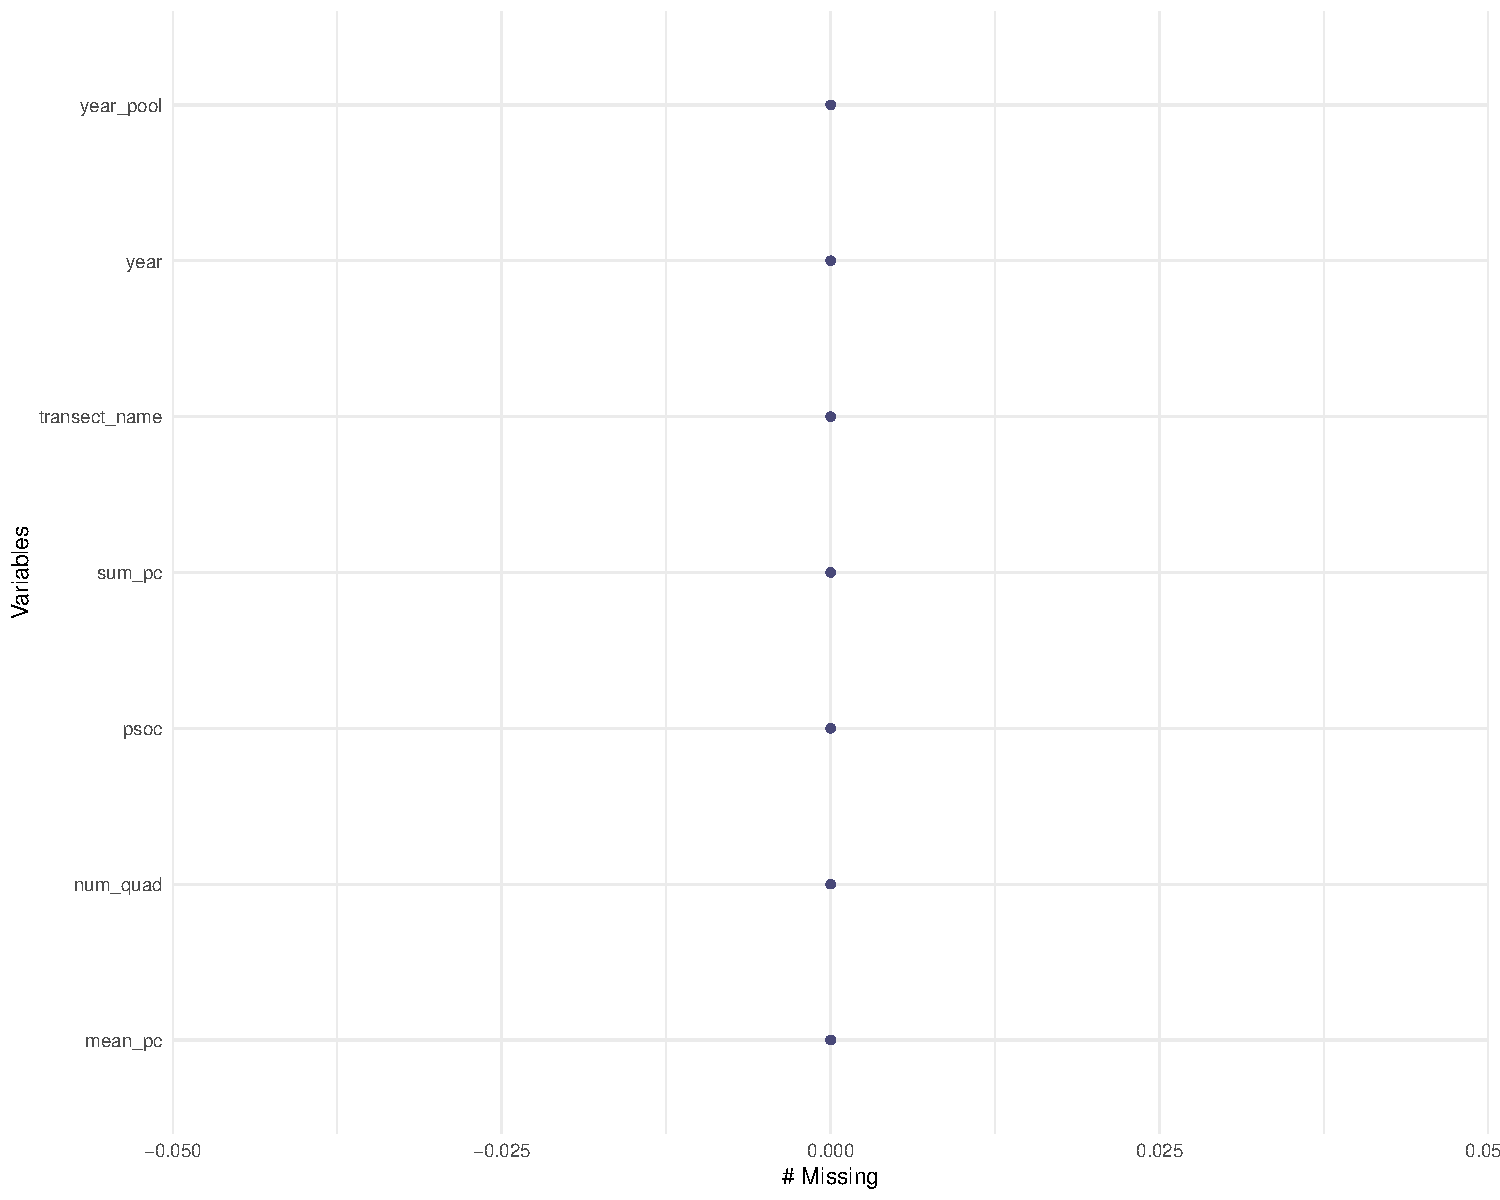
\includegraphics[keepaspectratio]{intermediate-elective2_files/figure-pdf/explicit 0s-1.pdf}}

\subsubsection{Create native and non-native
vectors}\label{create-native-and-non-native-vectors}

\begin{Shaded}
\begin{Highlighting}[]
\CommentTok{\# create a vector of native species names}
\NormalTok{native\_spp }\OtherTok{\textless{}{-}}\NormalTok{ veg }\SpecialCharTok{|\textgreater{}}
  
  \CommentTok{\# keep only native cover rows}
  \FunctionTok{filter}\NormalTok{(cover\_category }\SpecialCharTok{==} \StringTok{"NATIVE COVER"}\NormalTok{) }\SpecialCharTok{|\textgreater{}}
  
  \CommentTok{\# pull species column as a vector}
  \FunctionTok{pull}\NormalTok{(psoc) }\SpecialCharTok{|\textgreater{}}
  
  \CommentTok{\# keep only unique species names}
  \FunctionTok{unique}\NormalTok{()}


\CommentTok{\# create a vector of non{-}native species names}
\NormalTok{nonnative\_spp }\OtherTok{\textless{}{-}}\NormalTok{ veg }\SpecialCharTok{|\textgreater{}}
  
  \CommentTok{\# keep only non{-}native cover rows}
  \FunctionTok{filter}\NormalTok{(cover\_category }\SpecialCharTok{==} \StringTok{"NON{-}NATIVE COVER"}\NormalTok{) }\SpecialCharTok{|\textgreater{}}
  
  \CommentTok{\# pull species column as a vector}
  \FunctionTok{pull}\NormalTok{(psoc) }\SpecialCharTok{|\textgreater{}}
  
  \CommentTok{\# keep only unique species names}
  \FunctionTok{unique}\NormalTok{()}

\CommentTok{\# check number of species in each group}
\FunctionTok{length}\NormalTok{(native\_spp)}
\end{Highlighting}
\end{Shaded}

\begin{verbatim}
[1] 104
\end{verbatim}

\begin{Shaded}
\begin{Highlighting}[]
\FunctionTok{length}\NormalTok{(nonnative\_spp)}
\end{Highlighting}
\end{Shaded}

\begin{verbatim}
[1] 86
\end{verbatim}

\subsubsection{Add cover vectors to explicit
data}\label{add-cover-vectors-to-explicit-data}

\begin{Shaded}
\begin{Highlighting}[]
\CommentTok{\# add native/non{-}native grouping to explicit{-}zero data}
\NormalTok{cover\_explicit0 }\OtherTok{\textless{}{-}}\NormalTok{ pools\_explicit0 }\SpecialCharTok{|\textgreater{}}
  
  \CommentTok{\# create cover group based on species vectors}
  \FunctionTok{mutate}\NormalTok{(}\AttributeTok{cover\_group =} \FunctionTok{case\_when}\NormalTok{(}
\NormalTok{    psoc }\SpecialCharTok{\%in\%}\NormalTok{ native\_spp }\SpecialCharTok{\textasciitilde{}} \StringTok{"Native"}\NormalTok{,}
\NormalTok{    psoc }\SpecialCharTok{\%in\%}\NormalTok{ nonnative\_spp }\SpecialCharTok{\textasciitilde{}} \StringTok{"Non{-}native"}\NormalTok{,}
    \ConstantTok{TRUE} \SpecialCharTok{\textasciitilde{}} \ConstantTok{NA\_character\_}
\NormalTok{  )) }\SpecialCharTok{|\textgreater{}}
  
  \CommentTok{\# remove species that were not classified as native or non{-}native}
  \FunctionTok{filter}\NormalTok{(}\SpecialCharTok{!}\FunctionTok{is.na}\NormalTok{(cover\_group)) }\SpecialCharTok{|\textgreater{}}
  
  \CommentTok{\# keep columns needed for summarizing and plotting}
  \FunctionTok{select}\NormalTok{(year,}
\NormalTok{         transect\_name,}
\NormalTok{         psoc,}
\NormalTok{         cover\_group,}
\NormalTok{         sum\_pc,}
\NormalTok{         num\_quad,}
\NormalTok{         mean\_pc)}

\CommentTok{\# check grouped data}
\NormalTok{cover\_explicit0 }\SpecialCharTok{|\textgreater{}}
  \FunctionTok{slice\_sample}\NormalTok{(}\AttributeTok{n =} \DecValTok{10}\NormalTok{)}
\end{Highlighting}
\end{Shaded}

\begin{verbatim}
# A tibble: 10 x 7
    year transect_name psoc                  cover_group sum_pc num_quad mean_pc
   <dbl> <chr>         <chr>                 <chr>        <dbl>    <dbl>   <dbl>
 1  2022 VP-08         Pseudognaphalium_lut~ Non-native       0       17    0   
 2  2024 VP-07         Polypogon_interruptus Non-native       0       19    0   
 3  2024 VP-02         Melilotus_indicus     Non-native       0       19    0   
 4  2022 VP-08         Brassica_nigra        Non-native       0       17    0   
 5  2024 VP-07         Atriplex_prostrata    Non-native       0       19    0   
 6  2022 VP-01         Cotula_coronopifolia  Non-native       4       25    0.16
 7  2021 VP-03         Urospermum_piciroides Non-native       0       25    0   
 8  2023 VP-08         Trifolium_repens      Non-native       0       18    0   
 9  2024 VP-04         Parapholis_incurva    Non-native       0       20    0   
10  2023 VP-02         Bromus_diandrus       Non-native       0       19    0   
\end{verbatim}

\subsubsection{Summarize data}\label{summarize-data}

\begin{Shaded}
\begin{Highlighting}[]
\CommentTok{\# summarize native and non{-}native cover by year, pool, and cover group}
\NormalTok{cover\_pool\_year }\OtherTok{\textless{}{-}}\NormalTok{ cover\_explicit0 }\SpecialCharTok{|\textgreater{}}
  
  \CommentTok{\# group by year, pool, and cover group}
  \FunctionTok{group\_by}\NormalTok{(year, transect\_name, cover\_group) }\SpecialCharTok{|\textgreater{}}
  
  \CommentTok{\# calculate total mean percent cover across species}
  \FunctionTok{summarize}\NormalTok{(}\AttributeTok{total\_mean\_pc =} \FunctionTok{sum}\NormalTok{(mean\_pc, }\AttributeTok{na.rm =} \ConstantTok{TRUE}\NormalTok{),}
            \AttributeTok{.groups =} \StringTok{"drop"}\NormalTok{)}


\CommentTok{\# summarize average native and non{-}native cover across pools by year}
\NormalTok{cover\_year\_summary }\OtherTok{\textless{}{-}}\NormalTok{ cover\_pool\_year }\SpecialCharTok{|\textgreater{}}
  
  \CommentTok{\# group by year and cover group}
  \FunctionTok{group\_by}\NormalTok{(year, cover\_group) }\SpecialCharTok{|\textgreater{}}
  
  \CommentTok{\# calculate average cover across pools}
  \FunctionTok{summarize}\NormalTok{(}\AttributeTok{mean\_cover =} \FunctionTok{mean}\NormalTok{(total\_mean\_pc, }\AttributeTok{na.rm =} \ConstantTok{TRUE}\NormalTok{),}
            \AttributeTok{sd\_cover =} \FunctionTok{sd}\NormalTok{(total\_mean\_pc, }\AttributeTok{na.rm =} \ConstantTok{TRUE}\NormalTok{),}
            \AttributeTok{n\_pools =} \FunctionTok{n\_distinct}\NormalTok{(transect\_name),}
            \AttributeTok{.groups =} \StringTok{"drop"}\NormalTok{)}

\CommentTok{\# display summarized data}
\NormalTok{cover\_year\_summary}
\end{Highlighting}
\end{Shaded}

\begin{verbatim}
# A tibble: 10 x 5
    year cover_group mean_cover sd_cover n_pools
   <dbl> <chr>            <dbl>    <dbl>   <int>
 1  2021 Native            31.3    18.2        8
 2  2021 Non-native        13.8     7.63       8
 3  2022 Native            34.0    22.2        8
 4  2022 Non-native        26.7    16.7        8
 5  2023 Native            63.1    36.0        8
 6  2023 Non-native        34.8    22.8        8
 7  2024 Native            65.0    24.4        8
 8  2024 Non-native        37.9    16.1        8
 9  2025 Native            61.2    29.9        8
10  2025 Non-native        29.9     8.88       8
\end{verbatim}




\end{document}
